\documentclass{beamer}

\usepackage{../../../latex_style/beamerthemeExecushares}
\usepackage{../../../latex_style/notations}

\title{Session 13: Stochastic gradient descent}
\subtitle{Optimization and Computational Linear Algebra for Data Science}
\author{Léo Miolane}
\date{}

\setcounter{showSlideNumbers}{1}

\begin{document}

\setcounter{showProgressBar}{0}
\setcounter{showSlideNumbers}{0}

\frame{\titlepage}
\setcounter{framenumber}{0}
%\setcounter{showProgressBar}{1}
\setcounter{showSlideNumbers}{1}


\begin{frame}{Final exam}
	\begin{itemize}
		\item Scope: everything except today's lecture and this week's video.
			\vspace{1mm}
		\item Of course, it will be a bit more focused on what we did after the midterm (PCA, linear regression, convex functions, optimization...)
			\vspace{2mm}
		\item Same format as for the midterm
			\vspace{2mm}
		\item ``24 hours window'' on Thursday December 17th.
			\vspace{2mm}
		\item 1 hour 40 minutes to work + 20 minutes to scan + upload on Gradescope.
			\vspace{2mm}
		\item In case you have any issue when uploading: \textbf{email me your work}.
	\end{itemize}
\end{frame}

\begin{frame}
	\frametitle{Contents}
	\begin{enumerate}
		\item Introduction: supervised learning
		\item Stochastic gradient descent
		\item Convergence analysis, comparison with gradient descent
	\end{enumerate}
\end{frame}


\section{Introduction}


\begin{frame}[t]{Supervised learning}
	\grid

	\pause
	\pause

\end{frame}

\begin{frame}[t]{Why not using gradient descent ?}
	\grid
	$$
	f(\theta) = \frac{1}{N} \sum_{i=1}^N f_i(\theta).
	$$
	\vspace{-0.8cm}
	\begin{exampleblock}{}
		Gradient descent iterations:
\begin{align*}
	\theta_{t+1} 
	&= \theta_t - \alpha_t \nabla f(\theta_t) 
	\\
	&= \theta_t - \frac{\alpha_t}{N} \sum_{i=1}^N \nabla f_i(\theta_t).
\end{align*}
\vspace{-0.5cm}
	\end{exampleblock}

\end{frame}

\section{Stochastic gradient descent}

\begin{frame}[t]{Stochastic gradient descent}
	\grid
	$$
	f(\theta) = \frac{1}{N} \sum_{i=1}^N f_i(\theta).
	$$
	\vspace{-0.6cm}
	\begin{exampleblock}{}
		Starting at some $\theta_0 \in \R^n$, perform the updates:
\begin{align*}
	&\text{Pick} \quad i \quad \text{uniformly at random in} \quad \{1, \dots, N\}, \\
	&\text{Update} \quad \theta_{t+1} = \theta_t - \alpha_t \nabla f_i(\theta_t),
\end{align*}
	\end{exampleblock}

\end{frame}

\begin{frame}[t]{Tradeoffs in SGD}
	\grid

	\begin{columns}
		\begin{column}{0.45\textwidth}
			\vspace{-0.5cm}
			\begin{center}
				\textbf{Rapidly decaying step sizes}
			\end{center}
			\hspace*{-0.4cm}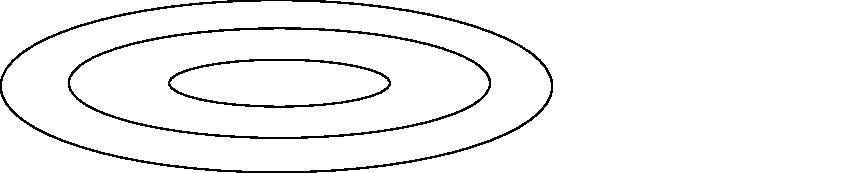
\includegraphics[width=9cm]{../figures/contour.pdf}
			\vspace{2.7cm}
	\end{column}
	\vrule
		\begin{column}{0.55\textwidth}
			\vspace{-0.5cm}
			\begin{center}
				\textbf{Slowly decaying step sizes}
			\end{center}
			\hspace*{0.4cm}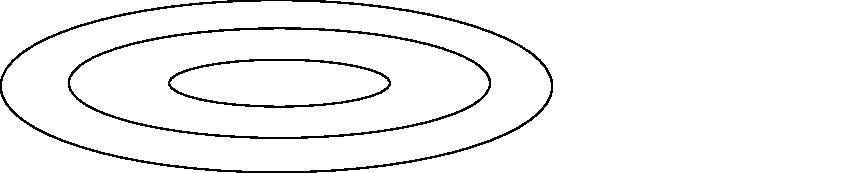
\includegraphics[width=9cm]{../figures/contour.pdf}
			\vspace{2.7cm}
	\end{column}
	\end{columns}

\end{frame}

\begin{frame}[t]{SGD in practice}
	\grid
	\vspace{-0.6cm}
	\begin{exampleblock}{}
		Mini-batch stochastic gradient descent:
\begin{align*}
	&\text{Pick a mini-batch} \quad i_1, \dots, i_k \quad \text{in} \quad \{1, \dots, N\}, \\
	&\text{Update} \quad \theta_{t+1} = \theta_t - \frac{\alpha_t}{k}\sum_{m=1}^k \nabla f_{i_m}(\theta_t),
\end{align*}
	\end{exampleblock}

	\begin{itemize}
		\item Decrease the step size after a fixed number of epochs.
		\item Use momentum + ``adaptive gradient'': Adagrad, RMSprop, Adedelta, Adam, Adamax, Nadam...
	\end{itemize}
	\vspace{0.3cm}

	Excellent reference:
	\begin{center}
		\url{https://arxiv.org/pdf/1609.04747.pdf}
	\end{center}

\end{frame}


\section{Convergence analysis}

\begin{frame}[t]{Convergence rates}
	\grid

	\begin{exampleblock}{}
		\begin{itemize}
			\item if the $f_i$ are convex and $L$-smooth: SGD with $\alpha_t = 1 / \sqrt{t}$ achieves an error $\leq C / \sqrt{t}$.
			\item if the $f_i$ are $\mu$-strongly convex and $L$-smooth: SGD with $\alpha_t = 1 / (\mu t)$ achieves an error $\leq C / t$.
		\end{itemize}
	\end{exampleblock}

\end{frame}


\begin{frame}[t]{GD \ vs \ SGD}
	\grid

	\begin{columns}
		\begin{column}{0.45\textwidth}
			\vspace{-0.5cm}
			\begin{center}
				\textbf{Gradient descent}
			\end{center}
			\begin{itemize}
				\item Time per step
			\vspace{1cm}
				\item Error after $t$ steps
			\vspace{2cm}
				\item Log-error after $\tau$ units of time
			\vspace{2cm}
			\end{itemize}
	\end{column}
	\vrule
		\begin{column}{0.55\textwidth}
			\vspace{-0.5cm}
			\begin{center}
				\textbf{Stochastic gradient descent}
			\end{center}
			\begin{itemize}
				\item Time per step
			\vspace{1cm}
				\item Error after $t$ steps
			\vspace{2cm}
				\item Log-error after $\tau$ units of time
			\vspace{2cm}
			\end{itemize}
	\end{column}
	\end{columns}

\end{frame}

\begin{frame}[t]{GD \ vs \ SGD}
	\grid

	\hspace*{-0.7cm}
	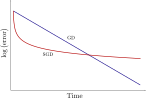
\includegraphics[width=12cm]{../figures/gd_sgd.pdf}

\end{frame}

\begin{frame}[t]{GD \ vs \ SGD: who wins ?}
	\grid

	\begin{itemize}
		\item If one is looking for a very small optimization error $f(\theta_t) - \min f$, then gradient descent wins.
			\vspace{2mm}
		\item If one has a limited time budget and does not need a very small $f(\theta_t) - \min f$, then stochastic gradient descent wins.
	\end{itemize}

\end{frame}

\appendix
\backupbegin

\begin{frame}[t]
	\frametitle{Questions?}
	\grid

	\pause
\end{frame}

\backupend



\end{document}
